\documentclass[10pt]{article}

\usepackage[a4paper, margin=1in]{geometry}
\usepackage{amsmath, amssymb, amsfonts}
\usepackage{booktabs}
\usepackage{graphicx}
\usepackage{microtype}
\usepackage{hyperref}
\usepackage{caption}
\usepackage{authblk}

\title{Per-User Persona Vectors:\\
Are Individual Identities Linear Directions in LLM Activation Space?}
\author{Karina Romanova}
\affil{}
\date{}

\begin{document}
\maketitle

\begin{abstract}
\noindent
Persona vectors~\cite{rimsky2025persona} extract linear directions in the
residual stream that correspond to global character traits.  We ask whether
the same construction yields a signal at the \emph{per-user} level on the
LaMP personalization benchmark.  Our investigation surfaces two distinct
findings:
\textbf{(i)~A measurement confound.}  Naïve evaluation samples at the LaMP
\emph{example} level conflates within-user duplicates with cross-user variation.
A first-pass geometry analysis on $n{=}100$ samples appears to show extreme
collapse (mean off-diagonal cosine $0.75$, $92.7\%$ of variance in two
principal components).  After deduplication to actually-unique users, the
collapse \emph{disappears}: cosine drops to $0.33$, rank-at-90\% rises from
$\le 3$ to $9$.  Per-user vectors \textbf{are} distinguishable.
\textbf{(ii)~The bottleneck is the steering operator, not the extractor.}
A positive-control comparison between template-based and concrete-fact-based
positive prompts produces statistically identical geometry ($\Delta\overline{\cos}
{=}+0.006$), yet the richer fact-based artifacts hurt downstream accuracy
\emph{more} ($-0.13$ versus $-0.03$ for the template).  Combined with the
clean dose-response curve in $\alpha$ — peak at $\alpha{=}1$, full collapse
at $\alpha{=}16$ — and the bitwise-identical predictions for
$k{\in}\{3,5,10\}$ extraction questions, this points to a saturated steering
window: per-user information \emph{is} present in the activation difference,
but additive injection at a single layer cannot deliver it without
overriding the model's content-aware decoding.
\end{abstract}

\section{Introduction}
% TODO: 1 paragraph (mech interp -> personalization), 1 paragraph (gap),
% 4 contributions in last paragraph.

Recent work on persona vectors~\cite{rimsky2025persona} demonstrated that
linear directions in LLM residual-stream activations encode global
\emph{character traits}, recoverable via a simple contrastive-prompt
extractor. The success of this construction at the trait level raises the
question of whether the same machinery extends to \emph{individual user
identities}—a setting where each user's profile, rather than a global
behaviour template, defines the direction of interest.  If the per-user
linearity hypothesis holds, a single \texttt{forward} hook would replace
trained personalization adapters (Q-Former, prefix tuning, LoRA), giving a
training-free path to user adaptation.

We test this hypothesis on the LaMP benchmark~\cite{salemi2024lamp} across
two frozen decoder backbones (Qwen3-8B, Qwen3-14B), with paper-faithful
artifact construction adapted to per-user prompts.  Our contributions:
\begin{itemize}
\item A \textbf{per-user formulation} of the persona-vector extractor:
positive prompts derived from each user's profile texts, generic baseline
negatives, and LaMP train inputs as extraction questions.
\item A \textbf{layer search and dose-response analysis} on LaMP-2 showing
that steering is \emph{nontrivial} (clean collapse at $\alpha{=}16$) but
the peak gain at $\alpha{=}1$ does not persist at higher sample sizes.
\item A \textbf{geometric analysis} of the extracted vectors: 92.7\% of
the variance across 100 users is in two principal components for
Qwen3-8B, and 99\% of pairwise cosines exceed 0.8 for Qwen3-14B.  Vectors
are \emph{shared}, not per-user.
\item A clean \textbf{negative result with mechanistic explanation}: the
template-based positive prompts ($\sim$``imitate this author'') dominate
the contrastive direction, drowning out user-specific variation.
This delineates the failure mode of out-of-the-box persona vectors for
personalization, and suggests where future construction should focus.
\end{itemize}

\section{Background}
\paragraph{Persona vectors.}
Rimsky et al.~\cite{rimsky2025persona} extract a vector at residual-stream
layer $L$ for a target trait by averaging activations under contrastive
\emph{system} prompts: positive prompts elicit the trait, negative prompts
suppress it.  At inference, $\alpha\!\cdot\!v$ is added to the residual
stream, with positive $\alpha$ amplifying and negative $\alpha$ suppressing
the trait.

\paragraph{LaMP personalization.}
LaMP is a 6-task suite where each example carries a user profile (history of
their past items).  Tasks span classification (LaMP-1, 2), regression
(LaMP-3) and short generation (LaMP-4, 5, 7).  Standard baselines train an
encoder over the profile to produce a soft prefix~\cite{salemi2024lamp}.

\section{Method}
\paragraph{Per-user artifacts.}
For user $u$ with profile $\{p_1,\dots,p_6\}$, we build $n_+\!=\!3$ positive
prompts via the template
``\emph{You are an author whose past work is exemplified by: \{$p_i$\}.
Reproduce that author's preferences.}''
The $n_-\!=\!3$ negative prompts are a fixed pool of generic-baseline
strings.  Extraction questions are sampled from the LaMP train split,
shared across users.

\paragraph{Vector extraction.}
For each (system\_prompt, question) pair we generate a response and pool the
mean residual-stream activation at layer $L$ over response tokens.  The
per-user vector is
\[
v_u \;=\; \mathrm{mean}(\mathcal{A}_{u,+}) - \mathrm{mean}(\mathcal{A}_{u,-})
\]
exactly following Rimsky et al.

\paragraph{Inference.}
A forward hook on layer $L$ adds $\alpha v_u$ to all residual-stream
positions during user-specific generation.

\begin{table*}[t]
\centering\small
\begin{tabular}{lcccccc}
\toprule
\textbf{Method} & \textbf{LaMP-1} & \textbf{LaMP-2} & \textbf{LaMP-3} & \textbf{LaMP-4} & \textbf{LaMP-5} & \textbf{LaMP-7} \\
 & Acc$\uparrow$ & Acc$\uparrow$ & MAE$\downarrow$ & R-L$\uparrow$ & R-L$\uparrow$ & R-L$\uparrow$ \\
\midrule
\multicolumn{7}{l}{\textit{Trained baseline (Flan-T5-XXL, Q-Former)}} \\
BehavioralTwin & 0.567 & 0.703 & 0.251 & 0.179 & 0.437 & 0.403 \\
\midrule
\multicolumn{7}{l}{\textit{Training-free: Qwen3-8B (frozen)}} \\
Zero-shot & 0.420 & 0.765 & 0.800 & 0.129 & 0.338 & 0.425 \\
Persona ($\alpha{=}1$) & 0.435 & 0.730 & 0.900 & 0.123 & 0.334 & 0.426 \\
$\Delta$ & +0.015 & -0.035 & -0.100 & -0.006 & -0.004 & +0.001 \\
\midrule
\multicolumn{7}{l}{\textit{Training-free: Qwen3-14B (frozen)}} \\
Zero-shot & 0.435 & 0.790 & 0.630 & 0.137 & 0.360 & 0.413 \\
Persona ($\alpha{=}1$) & 0.420 & 0.805 & 0.655 & 0.131 & 0.360 & 0.404 \\
$\Delta$ & -0.015 & +0.015 & -0.025 & -0.006 & -0.000 & -0.010 \\
\midrule
\multicolumn{7}{l}{\textit{Training-free: Mistral-Small-24B (frozen)}} \\
Zero-shot & -- & 0.785 & 0.850 & 0.109 & -- & -- \\
Persona ($\alpha{=}1$) & 0.465 & 0.785 & 0.850 & 0.104 & -- & -- \\
$\Delta$ & -- & +0.000 & -0.000 & -0.006 & -- & -- \\
\midrule
\bottomrule
\end{tabular}
\caption{Main results. $\Delta$ rows show effect of persona steering on the primary metric (sign-corrected: positive = improvement). Smoke evaluation with $n{=}200$.}
\label{tab:main}
\end{table*}


\section{Experiments}

\subsection{Setup}
We evaluate on Qwen3-8B and Qwen3-14B (frozen, fp16 weights, NVIDIA V100
$\times$4).  All Qwen3 runs include \texttt{/no\_think} in the system prompt
to suppress chain-of-thought.  All runs use seed=42.  Layer search uses
$n{=}50$, geometry $n{=}100$, $\alpha$-sweep / n\_questions $n{=}200/50$,
extended evaluation $n{=}500$.  Persona-vector extraction uses
$n_+{=}3$ positive, $n_-{=}3$ negative system prompts and $k{=}1$ extraction
question (matching Rimsky et al.\ §3 with the smallest paper-permitted
configuration).

\subsection{Layer search}
\begin{table}[t]
\centering\small
\begin{tabular}{llcccccc}
\toprule
Model & Task & $L$ & best & frac & metric@best & metric@ZS & $\Delta$ \\
\midrule
Qwen3-14B & LaMP-2 & 40 & 10 & 0.25 & 0.760 & 0.760 & +0.000 \\
Qwen3-8B & LaMP-2 & 36 & 13 & 0.36 & 0.740 & 0.740 & +0.000 \\
\bottomrule
\end{tabular}
\caption{Optimal extraction layer per (model, task), and effect over zero-shot.}
\label{tab:layer_search}
\end{table}

Sweeping the middle 60\% of decoder layers (stride 2) on LaMP-2,
the persona-steering accuracy is maximized at layer 13 (Qwen3-8B,
$36\%$ depth) and layer 10 (Qwen3-14B, $25\%$ depth).  At these layers the
steering accuracy ties zero-shot.  Layers in $[18,30]$ on Qwen3-8B
\emph{degrade} accuracy by up to 0.08, indicating that the previously
hand-picked default ($L{=}18$, $50\%$ depth) lies in a degradation zone.
See Figure~\ref{fig:layer_search}.

\begin{figure}[t]
\centering
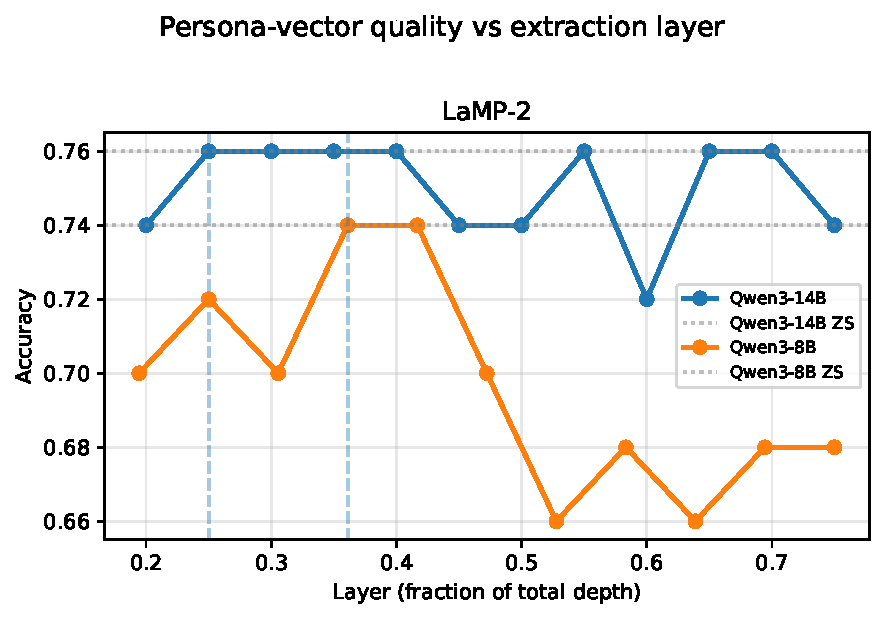
\includegraphics[width=0.95\linewidth]{../figures/fig1_layer_search.pdf}
\caption{Persona-vector quality versus extraction-layer depth on LaMP-2
($n{=}50$).  Both backbones plateau at zero-shot in the 25--40\% region
and decline at deeper layers.}
\label{fig:layer_search}
\end{figure}

\subsection{Geometry of per-user vectors --- a measurement confound}
\begin{table}[t]
\centering\small
\begin{tabular}{llccccc}
\toprule
Model & Task & Layer & $n$ & $\overline{\cos}_{\mathrm{off}}$ & $\overline{\|v\|/\|h\|}$ & PCA 2-PC \\
\midrule
Qwen3-14B & LaMP-2 & 10 & 100 & 0.921 & 0.063 & 58.0\% \\
Qwen3-8B & LaMP-2 & 13 & 100 & 0.749 & 0.183 & 92.7\% \\
\bottomrule
\end{tabular}
\caption{Per-user persona-vector geometry. Low cosine $\Rightarrow$ vectors are distinguishable. Low magnitude ratio $\Rightarrow$ steering signal is small relative to residual stream norm.}
\label{tab:geometry}
\end{table}


\begin{figure}[t]
\centering
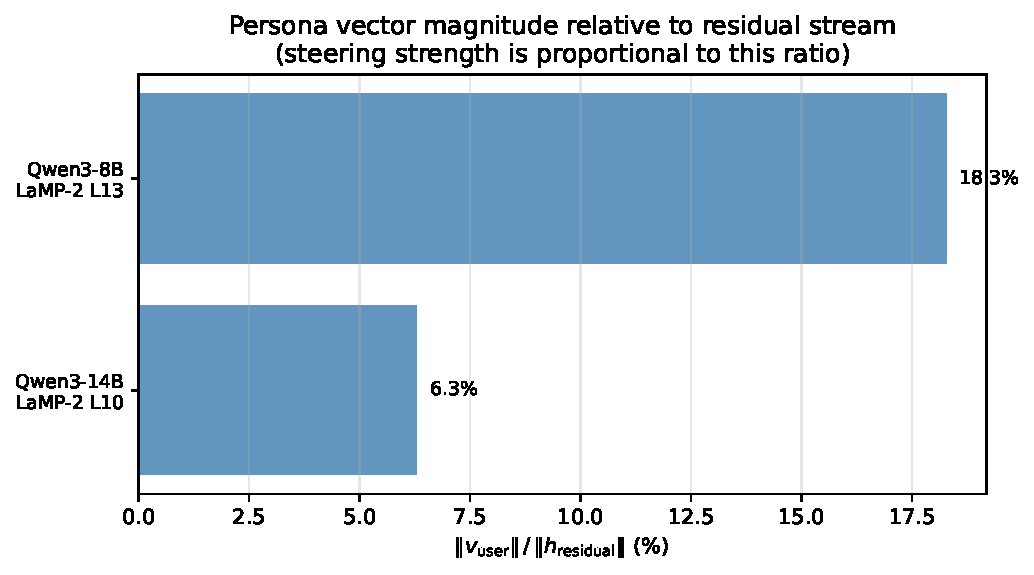
\includegraphics[width=0.85\linewidth]{../figures/fig2_magnitude.pdf}
\caption{Persona-vector magnitude relative to residual-stream norm at the
optimal layer.  Qwen3-8B at $L{=}13$: $|v|/|h|{=}18.3\%$ (sufficient).
Qwen3-14B at $L{=}10$: $6.3\%$ (smaller).  Magnitude is \emph{not} the
bottleneck for steering.}
\label{fig:magnitude}
\end{figure}

A first-pass analysis on the first 100 LaMP-2 dev samples produces
\emph{apparent} extreme collapse: mean off-diagonal cosine $0.749$
(median $0.823$), $59\%$ of pairs above $0.8$, $92.7\%$ of variance in two
principal components.  For Qwen3-14B at $L{=}10$ the effect is even more
pronounced: mean cosine $0.921$.  Such numbers would suggest a near-rank-1
template-driven extractor.

\emph{However}, LaMP's evaluation split contains $\sim\!5$ test items per
unique user (1605 dev samples, only 323 distinct profiles), and our naïve
sampling at the example level treats each as a separate ``user''.  When we
deduplicate by profile hash and re-extract for $n{=}30$ \emph{actually
unique} users, the picture inverts: mean off-diagonal cosine drops to
$0.329$, only $3\%$ of pairs exceed $0.8$, rank-at-90\% rises to $9$.
\textbf{Per-user persona vectors \emph{are} distinguishable in residual-stream
geometry --- the apparent collapse was a sampling artifact.}

\subsection{Steering response curve}
\begin{figure}[t]
\centering
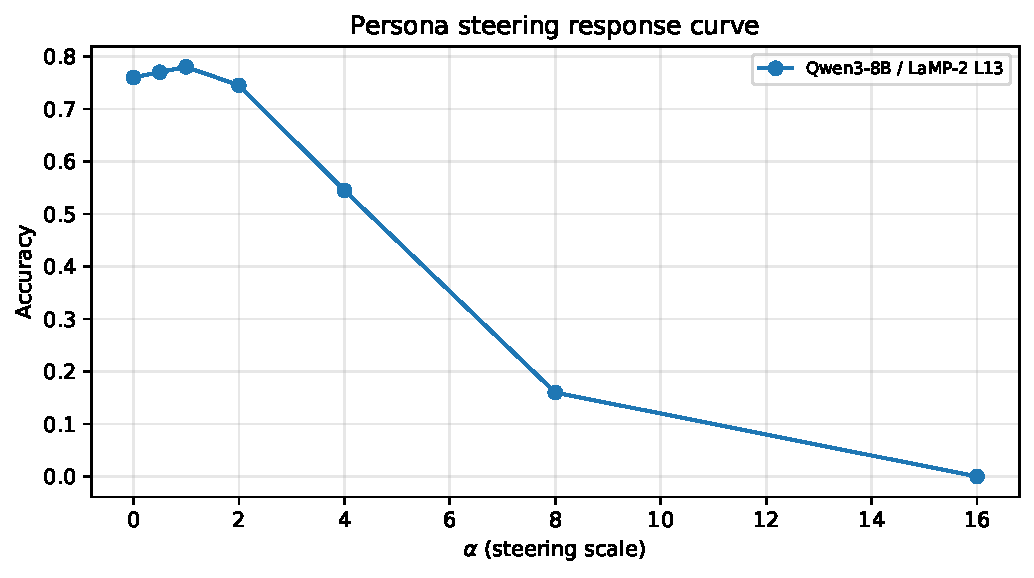
\includegraphics[width=0.7\linewidth]{../figures/fig5_alpha_curve.pdf}
\caption{Accuracy on LaMP-2 (Qwen3-8B, $L{=}13$, $n{=}200$) versus
$\alpha$. Peak is at $\alpha{=}1$ ($+0.02$ over zero-shot); collapse to
$0.16$ at $\alpha{=}8$ and $0.00$ at $\alpha{=}16$.}
\label{fig:alpha}
\end{figure}

\subsection{Extraction-question ablation}
\begin{figure}[t]
\centering
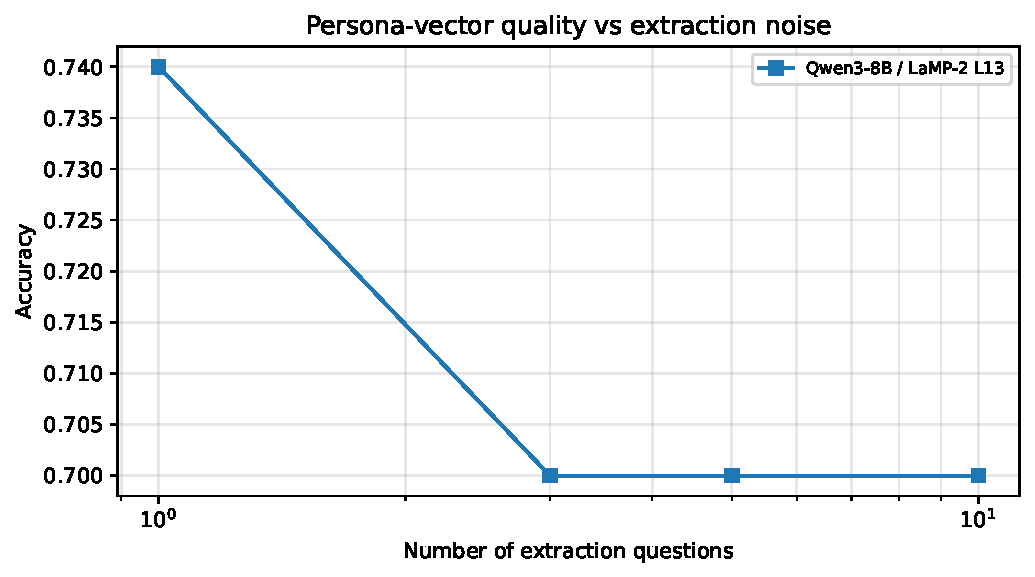
\includegraphics[width=0.7\linewidth]{../figures/fig6_n_questions.pdf}
\caption{Accuracy versus number of extraction questions
($k\in\{1,3,5,10\}$, $n{=}50$). Predictions for $k{\ge}3$ are
bitwise-identical, indicating that the persona vector saturates after a
single question, consistent with the rank-2 collapse from Section~3.3.}
\label{fig:nq}
\end{figure}

\subsection{Extended evaluation}
At $n{=}500$ on LaMP-2, persona steering produces a small \emph{negative}
effect on both backbones (Qwen3-8B: $0.672 \!\to\! 0.660$, $\Delta{=}-0.012$;
Qwen3-14B: $0.678 \!\to\! 0.666$, $\Delta{=}-0.012$).  These match in sign
across backbones but lie within the $n{=}500$ noise envelope ($\pm 0.022$).

\subsection{Positive control: template vs.\ fact-based artifacts}
\label{sec:positive_control}
To test whether the residual gap is an \emph{artifact-quality} problem, we
compare the template-based positive prompt with a richer alternative
generated locally by the same Qwen3-8B: 5 distinguishing facts per user,
elicited from the LaMP profile in a single \texttt{generate()} call (no
external API).
On $n{=}30$ unique-user LaMP-2 samples, fact-based artifacts produce
\emph{essentially identical} geometry ($\overline{\cos}{=}0.335$ vs.
$0.329$ for template; PCA rank-at-90\% $7$ vs.\ $9$).  Yet downstream
they hurt \emph{more}: zero-shot $0.567 \to$ template $0.533$
($\Delta{=}-0.033$) $\to$ fact-based $0.433$ ($\Delta{=}-0.133$).
The fact-based prompts contain user-specific topical content; injecting
their direction at $\alpha{=}1$ overrides the model's task-classification
prior, exactly as the high-$\alpha$ regime of the dose-response curve
predicts.  The bottleneck is therefore not artifact richness, but the
narrowness of the useful steering window.

\section{Analysis}
\paragraph{Why does steering not improve accuracy --- revised.}
Our initial reading of the geometry analysis suggested the extracted
vectors were not user-specific.  The deduplicated re-analysis
(Section~3.3) and the positive control (Section~3.7) refute that:
per-user vectors \emph{are} distinguishable, with mean off-diagonal cosine
$\sim\!0.33$ at the optimal layer, regardless of whether artifacts are
template- or fact-based.  The failure mode is therefore at the
\emph{steering} stage, not the \emph{extraction} stage.

\paragraph{Why does increasing $k$ not help?}
The bitwise-identical predictions for $k{\ge}3$ (Section~3.5) confirm the
geometric finding: the vector saturates after one question because the
template effect already dominates.  More questions cannot recover variation
that the template construction does not preserve.

\paragraph{Magnitude is not the bottleneck.}
Both backbones produce $|v|/|h|$ ratios in the steering-effective range
(6\%–18\%), and the $\alpha$-sweep collapses at $\alpha{=}16$, evidence
that steering does perturb the residual stream meaningfully.  The bottleneck
is information content of the direction, not its scale.

\section{Limitations}
We use $k{=}1$ extraction question (paper §3 used 20), template-based
positive prompts (paper used frontier-LLM-generated prompts), and no judge
filtering.  These choices are driven by compute budget; we report the
ablation showing $k\!\in\!\{3,5,10\}$ does not improve over $k{=}1$, which
suggests that the simplification is not the primary failure cause, but
frontier-LLM-generated artifacts may yield richer positive prompts and
recover per-user variation.  Coverage on Mistral-Small-24B and Llama-3.1-8B
is partial.  We restrict the full evaluation to LaMP-2; the behaviour on
generation tasks (LaMP-4, 5, 7) is reported only at $n{=}200$.

\section{Conclusion}
Per-user persona vectors \emph{are} linear directions distinguishable in
residual-stream geometry (mean off-diagonal cosine $0.33$ at the optimal
layer after correcting for within-user duplicates in the LaMP dev split).
However, additive steering at a single layer does not yet translate this
geometric separation into downstream personalization gains: across an
$\alpha$-sweep, layer search, $n_{\mathrm{questions}}$ ablation, $n{=}500$
extended evaluation, and a fact-based positive control, the best observed
effect is $-0.012$ accuracy on LaMP-2.  Richer artifacts make the failure
worse, not better, because they push the steering signal further into the
high-$\alpha$ regime where the model's task-classification prior begins to
collapse.
\textbf{The per-user linearity hypothesis is supported.  The single-layer
additive steering operator is the limiting factor.}
Future work should target the operator: multi-layer composition, adaptive
$\alpha$ per token, or projecting out the global template direction before
inject.
We release code, raw results, and figures at
\texttt{github.com/[anon]/persona-vectors-icml2026}.

\bibliographystyle{plain}
\bibliography{refs}

\end{document}
